\chapter{Un système de détection omnidirectionnel en temps réel}

	\section{Analyse du besoin}

		\subsection{Le concept du système}
			
			% Idée globale du système
			Le projet vise à créer un démonstrateur d'un concept plus large, à savoir un système permettant de piloter un ensemble de robots et d'exploiter les informations issues de leurs périphériques de capture afin d'effectuer des missions de reconnaissance sans déployer de troupes au sol, et risquer de mettre leurs vies en dangers sur des terrains potentiellement à risques. Ce démonstrateur illustre donc la faisabilité de ce concept, mais d'une manière plus limitée. Le but est de développer un système opérationnel pour un seul robot équipé d'un \gls{lidar} et d'une caméra sphérique, permettant de contrôler ses déplacements, d'analyser les données acquises par ces deux périphériques, et d'afficher les résultats de ces traitements dans une interface utilisateur.
			\par
			% Mon sujet de stage
			Devant l'ampleur du travail à accomplir, le projet a été scindé en deux sujets de stage, chacun correspondant au traitement des données acquise par un des deux périphériques. Le sujet dont il est question dans ce document est relatif à l'exploitation de la caméra sphérique. On dégage trois objectifs principaux à la mission décrite dans le sujet du stage:
			\begin{itemize}[noitemsep]
				\item Réalisation d'un état de l'art permettant de choisir le matériel et l'algorithme à utiliser.
				\item Développement d'une brique logicielle permettant d'effectuer de la reconnaissance d'objets en temps réel.
				\item Développement d'une brique logicielle permettant d'afficher les résultats de la détection incrustés à la vidéo.
			\end{itemize}
			\par
			Préalablement à la conception architecturale du projet, un document de \improvement{ajouter ref annexe + corriger STBL}\emph{Spécification Technique du Besoin Logiciel (STBL)} a été réalisé afin de détailler ces trois objectifs et de référencer les exigences de qualité. A cette occasion, des éléments d'analyse fonctionnelle ont été menés afin de mieux cerner le besoin. Le diagramme de cas d'utilisation suivant (\autoref{fig:usecase}) définit les exigences fonctionnelles et le cadre du projet d'un point de vue de l'utilisateur.
			
			\begin{figure}[h]
			{
				\centering
				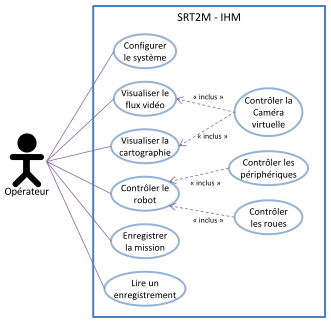
\includegraphics[page=1,width=0.7\textwidth]{figures/usecase.pdf}
				\caption{Diagramme de cas d'utilisation de l'interface homme-machine}
				\label{fig:usecase}
			}
			\end{figure}

			\improvement[inline]{Ajouter justification des technos employées}


		\subsection{Exigences}

			Le document de Spécification Technique du Besoin Logiciel développe le fonctionnement de la brique logicielle en trois fonctions principales détaillées dans la liste suivante, accompagnées de leurs descriptions:
			\begin{description}[noitemsep, before={\setcounter{descriptcount}{0}},font=\bfseries\stepcounter{descriptcount}\thedescriptcount.~]
				\item[Acquisition Vidéo:] Acquérir un flux vidéo provenant d’une caméra \oldstylenums{360}\degre.
				\item[Détection:] Détecter et classifier les objets d’intérêt présents dans le flux vidéo.
				\item[Retour visuel:] Offrir un retour visuel à l’opérateur présentant le flux vidéo et les objets détectés.
			\end{description}
			Ce document précise ces fonctions en y faisant correspondre des facteurs de qualité, appelés \emph{exigences fonctionnelles} qui permettent de piloter la réalisation du produit présentant ces fonctionnalités. Elles sont recensées dans les tableaux suivants avec leur référence, leur intitulé et une courte description:
			
			\begin{center}
	\begin{tabularx}{\textwidth}[t]{rsb}

		\arrayrulecolor{green}\hline
		\multicolumn{3}{c}{\textbf{\textcolor{myGreen}{FNC001-ACQUISITION\_VIDEO}}}\\
		\hline

		\textbf{Référence} & \textbf{Intitulé} & \textbf{Description} \\
		\arrayrulecolor{black}\hline
		
		FNC001\_01 & Décoder le flux vidéo & Le flux doit être décomposé en images séparées au format RGB8 \\
		\arrayrulecolor{gray}\hline
		FNC001\_02 & Transmettre séquentiellement les images obtenues du décodage & Les images décodées doivent être mises à disposition des fonctions dépendantes (détection et retour visuel) dans l’ordre d’obtention et sans latence supérieure à la vitesse d’acquisition. \\
		\arrayrulecolor{gray}\hline
		FNC001\_03 & Transmettre un horodatage relatif à une image décodée & Chaque image mise à disposition doit être accompagnée d’un horodatage permettant de la situer dans le temps de manière cohérente. \\
		\arrayrulecolor{gray}\hline
		FNC001\_04 & Relayer l’état du matériel et de la connexion & Les informations suivantes doivent être mises à disposition de la fonction retour visuel: Caméra connectée, flux vidéo disponible, erreur de décodage \\
		\arrayrulecolor{gray}\hline
		FNC001\_05 & Traiter les éventuelles erreurs de décodage & Les erreurs temporaires ne doivent pas affecter le fonctionnement du logiciel. En cas d’erreur, la relayer au retour visuel. \\
		\arrayrulecolor{gray}\hline

		\arrayrulecolor{green}\hline
		\multicolumn{3}{c}{\textbf{\textcolor{myGreen}{FNC002-DETECTION}}}\\
		\hline

	\end{tabularx}

	\begin{tabularx}{\textwidth}[t]{rsb}

		\textbf{Référence} & \textbf{Intitulé} & \textbf{Description} \\
		\arrayrulecolor{black}\hline
		
		FNC001\_01 & Décoder le flux vidéo & Le flux doit être décomposé en images séparées au format RGB8 \\
		\arrayrulecolor{gray}\hline
		FNC001\_02 & Transmettre séquentiellement les images obtenues du décodage & Les images décodées doivent être mises à disposition des fonctions dépendantes (détection et retour visuel) dans l’ordre d’obtention et sans latence supérieure à la vitesse d’acquisition. \\
		\arrayrulecolor{gray}\hline
		FNC001\_03 & Transmettre un horodatage relatif à une image décodée & Chaque image mise à disposition doit être accompagnée d’un horodatage permettant de la situer dans le temps de manière cohérente. \\
		\arrayrulecolor{gray}\hline
		FNC001\_04 & Relayer l’état du matériel et de la connexion & Les informations suivantes doivent être mises à disposition de la fonction retour visuel: Caméra connectée, flux vidéo disponible, erreur de décodage \\
		\arrayrulecolor{gray}\hline
		FNC001\_05 & Traiter les éventuelles erreurs de décodage & Les erreurs temporaires ne doivent pas affecter le fonctionnement du logiciel. En cas d’erreur, la relayer au retour visuel. \\
		\arrayrulecolor{gray}\hline
		
	\end{tabularx}

	\begin{tabularx}{\textwidth}[t]{rsb}

		\arrayrulecolor{green}\hline
		\multicolumn{3}{c}{\textbf{\textcolor{myGreen}{FNC003-RETOUR\_VISUEL}}}\\
		\hline

		\textbf{Référence} & \textbf{Intitulé} & \textbf{Description} \\
		\arrayrulecolor{black}\hline
		
		FNC001\_01 & Décoder le flux vidéo & Le flux doit être décomposé en images séparées au format RGB8 \\
		\arrayrulecolor{gray}\hline
		FNC001\_02 & Transmettre séquentiellement les images obtenues du décodage & Les images décodées doivent être mises à disposition des fonctions dépendantes (détection et retour visuel) dans l’ordre d’obtention et sans latence supérieure à la vitesse d’acquisition. \\
		\arrayrulecolor{gray}\hline
		FNC001\_03 & Transmettre un horodatage relatif à une image décodée & Chaque image mise à disposition doit être accompagnée d’un horodatage permettant de la situer dans le temps de manière cohérente. \\
		\arrayrulecolor{gray}\hline
		FNC001\_04 & Relayer l’état du matériel et de la connexion & Les informations suivantes doivent être mises à disposition de la fonction retour visuel: Caméra connectée, flux vidéo disponible, erreur de décodage \\
		\arrayrulecolor{gray}\hline
		FNC001\_05 & Traiter les éventuelles erreurs de décodage & Les erreurs temporaires ne doivent pas affecter le fonctionnement du logiciel. En cas d’erreur, la relayer au retour visuel. \\
		\arrayrulecolor{gray}\hline

	\end{tabularx}
\end{center}

			\bigskip

			La spécification technique décrit aussi d'autres contraintes de réalisation et de qualité, plus décorrélées de l'expression du besoin, qui auront un impact sur les décisions de conception et d'architecture du produit final. Pilotant l'ensemble de la réalisation, elles ne disposent pas de fonctions précises qui leur répondent, et de ce fait n'ont pas de référence. Ces contraintes sont énumérées dans les tableaux suivants:
			
			\begin{center}
	\scriptsize
	\begin{tabularx}{\textwidth}[t]{rsb}
		\arrayrulecolor{siiorange2}\cmidrule(l){1-3}
		\multicolumn{3}{c}{\textbf{\textcolor{siiorange}{Contraintes d'environnement}}}\\
		\arrayrulecolor{siiorange2}\cmidrule(l){1-3}

		\textbf{Type} & \textbf{Élément} & \textbf{Composants} \\
		\arrayrulecolor{black}\cmidrule(l){1-3}
		
		\multirow{4}{*}{Matériel} & \multirow{2}{*}{Plateforme mobile} & Raspberri Pi 3b \\ \arrayrulecolor{gray}\cmidrule(l){3-3}
		                          &                                    & périphérique d’acquisition de flux vidéo \\ \arrayrulecolor{gray}\cmidrule(l){2-3}
		                          & \multirow{2}{*}{Poste de contrôle} & Périphériques d'interface \\ \arrayrulecolor{gray}\cmidrule(l){3-3}
		                          &                                    & Processeur graphique \\ \arrayrulecolor{gray}\cmidrule(l){1-3}
		\multirow{7}{*}{Logiciel} & \multirow{3}{*}{Plateforme mobile} & Noyau linux (ARM) \\ \arrayrulecolor{gray}\cmidrule(l){3-3}
		                          &                                    & Outils GNU \\ \arrayrulecolor{gray}\cmidrule(l){3-3}
		                          &                                    & Framework ROS \\ \arrayrulecolor{gray}\cmidrule(l){2-3}
		                          & \multirow{4}{*}{Poste de contrôle} & Noyau Linux (x86-64) \\ \arrayrulecolor{gray}\cmidrule(l){3-3}
		                          &                                    & Outils GNU \\ \arrayrulecolor{gray}\cmidrule(l){3-3}
		                          &                                    & Framework ROS \\ \arrayrulecolor{gray}\cmidrule(l){3-3}
		                          &                                    & CUDA \\ \arrayrulecolor{gray}\cmidrule(l){1-3}
	\end{tabularx}
	
	\begin{tabularx}{\textwidth}[t]{rsb}
		\arrayrulecolor{siigreen2}\cmidrule(l){1-3}
		\multicolumn{3}{c}{\textbf{\textcolor{siigreen}{Contraintes d'interface}}}\\
		\arrayrulecolor{siigreen2}\cmidrule(l){1-3}

		\textbf{Type} & \textbf{Élément} & \textbf{Détails} \\
		\arrayrulecolor{black}\cmidrule(l){1-3}
		
		\multirow{4}{*}{Matériel} & \multirow{4}{*}{Périphérique d'acquisition vidéo} & Connection \gls{usb} 3.0\\ \arrayrulecolor{gray}\cmidrule(l){3-3}
								  &                                                   & Format vidéo \gls{mjpeg} \\ \arrayrulecolor{gray}\cmidrule(l){3-3}
								  &                                                   & Protocole \gls{uvc} \\ \arrayrulecolor{gray}\cmidrule(l){3-3}
								  &                                                   & Format d'image "Dual Fisheye" \\ \arrayrulecolor{gray}\cmidrule(l){1-3}
		\multirow{6}{*}{Logiciel} & \multirow{6}{*}{Système Robotique}                & Interface avec \gls{ros} \\ \arrayrulecolor{gray}\cmidrule(l){3-3}
								  &                                                   & Execution simultanée (les traitements ne doivent pas bloquer le reste du système) \\ \arrayrulecolor{gray}\cmidrule(l){3-3}
								  &                                                   & Latence minime dans le transfert d'images (<200ms) \\ \arrayrulecolor{gray}\cmidrule(l){3-3}
								  &                                                   & Transfert des détections synchronisé avec les images \\ \arrayrulecolor{gray}\cmidrule(l){3-3}
								  &                                                   & Transfert des données selon un protocole à définir \\ \arrayrulecolor{gray}\cmidrule(l){1-3}
	\end{tabularx}

	\begin{tabularx}{\textwidth}[t]{sb}
		\arrayrulecolor{siipurple2}\cmidrule(l){1-2}
		\multicolumn{2}{c}{\textbf{\textcolor{siipurple}{Contraintes de programmation}}}\\
		\arrayrulecolor{siipurple2}\cmidrule(l){1-2}

		\textbf{Élément} & \textbf{Valeur} \\
		\arrayrulecolor{black}\cmidrule(l){1-2}
		
		\multirow{1}{*}{Langages}   & C++ \\ \arrayrulecolor{gray}\cmidrule(l){1-2}
		\multirow{3}{*}{Frameworks} & \gls{cuda} \\ \arrayrulecolor{gray}\cmidrule(l){2-2}
								    & Qt5 \\ \arrayrulecolor{gray}\cmidrule(l){2-2}
									& \gls{ros} \\ \arrayrulecolor{gray}\cmidrule(l){1-2}
	\end{tabularx}
	
\end{center}

			
			\improvement[inline]{Ajouter du contenu ?}

	\section{Etat de l'art}

		\subsection{Détection d'objets et apprentissage automatique}
			
			La détection d'objets d'intérêt est une discipline de la vision par ordinateur qui consiste à détecter la présence d'un type d'objet (appelé communément \emph{classe}) dans une image. On peut distinguer plusieurs problématiques issues du sujet:
			\begin{description}[noitemsep]
				\item[Localisation:] Trouver les coordonnées exactes d'un objet dans une image.
				\item[Classification:] Associer une image contenant un objet à un élément d'un ensemble de classes prédéfinies.
				\item[Reconnaissance:] Identifier une instance précise d'une classe (distinguer deux éléments distincts de même classe).
			\end{description}
			Pour répondre à ces problématiques, on utilise généralement un \emph{système de reconnaissance de forme}, procédé permettant de décrire une image ou partie d'une image au travers d'une représentation mathématique et de la comparer à des modèles de représentations connus afin de l'assimiler à une classe définie. Un des exemples les plus connus est la \emph{Méthode de Viola et Jones}\cite{viola}, principalement utilisée pour la détection de visages. Ces systèmes comprennent deux éléments principaux:
			\begin{itemize}[noitemsep]
				\item Un extracteur des caractéristiques de l'entrée
				\item Un classifieur qui associe l'entrée à une classe
			\end{itemize}
			\par
			L'extracteur de caractéristiques est un algorithme qui permet de traduire une image, ou partie d'une image, en une représentation mathématique de caractéristiques visuelles qu'elle contient (coins, traits, points, dégradés \dots). L'approche classique consiste à considérer l'entrée comme un élément d'un espace vectoriel de dimension $n_{0}$ et d'y appliquer une fonction mathématique pour obtenir un résultat appartenant à un espace vectoriel de dimension $n_{1}$ avec $n_{1} < n_{0}$, qu'on appelle \emph{vecteur de caractéristiques} ou \emph{descripteur}. L'intérêt de ces traitements réside dans cette réduction de dimensions, qui constitue en quelque sorte un résumé de la donnée, et permet de distinguer plus facilement des classes grâce à l'algorithme de classification. Il existe de nombreux algorithmes extracteurs de caractéristiques, autant qu'il existe de nombreux moyens de décrire les caractéristiques visuelles d'une image. Citons les algorithmes \emph{SIFT}\cite{sift}, \emph{HOG}\cite{hog} et \emph{SURF}\cite{surf} comme exemples, par leur utilisation régulière dans la communauté du traitement du signal. Contrairement au classifieur, ces algorithmes sont fixes, c'est à dire que pour une même entrée, ils produiront toujours la même sortie.
			\par
			Le classifieur, souvent basé sur des \emph{Machines à Vecteur de Support}\cite{svm}, permet de discriminer des groupes au sein des résultats, et donc de déterminer l'appartenance d'un résultat à une classe. Afin de déterminer la classe résultante d'un objet ($y_{i}$), il effectue des sommes pondérées des composantes de ses vecteurs de caractéristiques, et les compare à des valeurs seuils permettant d'activer ou non une sortie. Un algorithme classifieur est généralement entraînable, c'est à dire qu'en lui fournissant un ensemble de couples (vecteurs de caractéristiques; résultat attendu $\hat{y}_{i}$) il déterminera lui même la loi permettant de les séparer. L'enjeu est de réduire l'écart entre $y$ et $\hat{y}$, cette phase d'entraînement revient donc à minimiser une fonction objectif en modulant les pondérations des sommes ($\theta_{i}$) jusqu'à obtenir une loi de discrimination optimale. Un tel comportement correspond à un apprentissage supervisé, où la réponse correcte est connue, permettant à la machine de s'améliorer. Une fois cette phase achevée, le système est théoriquement apte à classifier avec exactitude de nouvelles entrées, jusqu'alors inconnues.

		\subsection{Apprentissage profond et R-CNN}

			L'apprentissage profond est basé sur l'utilisation de réseaux neuronaux artificiels multicouche. Ces réseaux sont schématiquement inspirés des réseaux neuronaux biologiques tels que nous les connaissons en ceci qu'ils se basent sur la transmission de données entre de nombreux modules, appelés \emph{Neurones Formels}, illustré en \autoref{fig:aneuron}. Ces modules prennent en entrée $x_{i}$ des valeurs issues des résultats de neurones précédents ou bien de l'entrée d'origine du système. Ces entrées sont ensuite sommées avec leur \emph{poid synaptique} $\theta_{i}$ respectif, ainsi qu’un coefficient $\theta_{0}$ appelé biais. Ce résultat pondéré est ensuite transmis à une fonction d’activation non linéaire. Celle-ci activera la synapse suivante (ici, la sortie), si son résultat dépasse un seuil donné.
			\begin{figure}[h]
			{
				\centering
				\includegraphics[page=1,width=.6\textwidth]{figures/aneuron.pdf}
				\caption{Schéma d'un neurone formel}
				\label{fig:aneuron}
			}
			\end{figure}
			
			
			\info[inline]{WIP}

		\subsection{Vidéo sphérique}
			% de 1 à 36 objectifs
			La photographie sphérique, aussi connue sous le nom de photographie à 360\degre ou \emph{VR photography} (pour réalité virtuelle), s'apparente à la photographie panoramique, en ceci qu'elle vise à capturer un point de vue sous la forme d'une image avec un champ de vision exceptionnellement large (ratio supérieur à $1:2$)\cite{fnumpano}. En effet, le but est de représenter une scène complète dans une seule image, comme on pourrait l'observer en effectuant un tour complet autour d'un point fixe. Le concept s'est fortement démocratisé au travers de son apparition dans \emph{Google StreetView}, et plus récemment par l'importante médiatisation de la réalité virtuelle, permettant une plus grande immersion lors du visionnage de photographies ou de vidéos sphériques.
			\par
			L'obtention d'une image prête au visionnage n'est théoriquement pas possible avec une seule prise de vue. Les techniques utilisées pour obtenir de telles images reposent toutes sur l'assemblage de plusieurs photographies, ce qui peut faire apparaître des incohérences dans la scène lorsqu'elles sont prises à des temps différents (les sujets qui se déplacent peuvent être présents sur plusieurs photographies, donc plusieurs parties de la scène). Pour obtenir le plus de cohérence dans le flux vidéo et minimiser le traitement dû à l'assemblage, il a donc été décidé d'acquérir un appareil qui permet de capturer instantanément une scène complète avec plusieurs objectifs.
			\improvement[inline]{Ajouter images ou schémas}
			\par
			Cette médiatisation importante de la réalité virtuelle a entraîné la conception de caméras à \oldstylenums{360}\degre par de nombreux fabricants grand-public (LG, Samsung, Kodak), par opposition aux fabricants de matériel vidéo professionnel, comme FLIR (avec sa série des \emph{Ladybug} \cite{ladybug}). La recherche de matériel à acquérir s'est donc concrétisée par la création d'un comparatif des différentes caméras à \oldstylenums{360}\degre présent dans l'annexe \todoref.
			
			Le choix d'acquisition du matériel à été piloté principalement par les facteurs suivants:
			\begin{itemize}[noitemsep]
				\item Couverture spatiale complète ($360^{\circ}\times180^{\circ}$)
				\item Au moins \oldstylenums{15} images/secondes
				\item Transmission de la vidéo par WiFi ou USB
				\item Transmission de la capture vidéo en temps réel
				\item Assemblage d'image en temps réel
				\item Qualité d'image correcte (subjectif)
				\item Point de montage par vis
				\item Prix ne dépassant pas 500\euro
			\end{itemize}
			
			Notre choix s'est d'abord porté sur le produit Insta\oldstylenums{360} 4K\cite{insta360}, qui possède un système d'assemblage en temps réel intégré et une très bonne qualité d'image. Cependant, le produit n'étant pas disponible au moment de l'achat, nous avons dûs nous reporter sur la caméra Theta S de Ricoh\cite{ricohthetas}, possédant une qualité d'image moindre et aucun moyen natif d'assemblage en temps réel sous systèmes linux. Ce dernier point s'est avéré crucial dans l'organisation du travail, car il a nécessité une charge de travail importante, détaillée en \ref{sub:transfo}.

	\section{Problématiques soulevées}

		\subsection{Détection sur une image déformée}

			\content[inline]{A faire}

		\subsection{Visualisation des résultats}

			\content[inline]{A faire}
		
			
